% main.tex, to be used with thesis.tex
% This contains the main work of your thesis.

%\bibliography{thesis}  % uses the references stored in Chapter1Radar.bib

\chapter{DSP Data Persistence: Component Implementation}

This section shows the implementation of the DSP Data Persistence, which
follows the specifications of the DSP Components in the previous chapter,
along with the setup of the mongoDB, the chosen database system that models
data in a type of key-value pair model. Moreover, this chapter also describes
the experiments conducted for the persistence.

The implementation of the DSP Data Persistence component, as well as the
implementation of the experiments, were developed and managed using the DSP a
reserved development branch at the Subversion \cite{subversion} repository
located at the Google Code website. In this way, anyone can checkout the entire
source-code from the branch
\textit{https://netbeams.googlecode.com/svn/branches/marcello/persistence},
as shown in Figure \ref{fig:dsp-data-persistence-dir}. In this way, the
recommended checkout branch directory will give the remaining directory
structure as summarized:

\begin{itemize}
  \item \textbf{NEBEAMS-DIR/}: the directories under the subdirectory
  ``persistence'';
  \item \textbf{DEV-VERSION}: the directory of the current development
  version for the DSP; That is, ``\textbf{NEBEAMS-DIR}/versions/v2/''
  \item \textbf{PERSISTENCE-DIR}: the directory of the DSP component, that is,
  ``\textbf{DEV-VERSION}/apps/osgi-intro-bundles/dsp/DSPDataPersistence''.
\end{itemize}

\begin{figure}[!b]
  \centering
  \includegraphics[scale=0.6]{../diagrams/dsp-data-persistence-dir}
  \caption{The DSP Data Persistence Directory Structure}
  \label{fig:dsp-data-persistence-dir}
\end{figure}

The DSP Platform defines its own run-time directory, which organizes the
artifacts used by the osgi-intro Framework, as well as the its own configuration
descriptor and matcher, as described in the previous section. 

\begin{itemize}
  \item \textbf{RUNTIME-DIR}: the main directory for the execution of the DSP
Platform, with all the necessary osgi-intro-related artifacts are placed, as shown in
Figure \ref{fig:dsp-runtime-dir}.
\end{itemize}

\begin{figure}[!t]
  \centering
  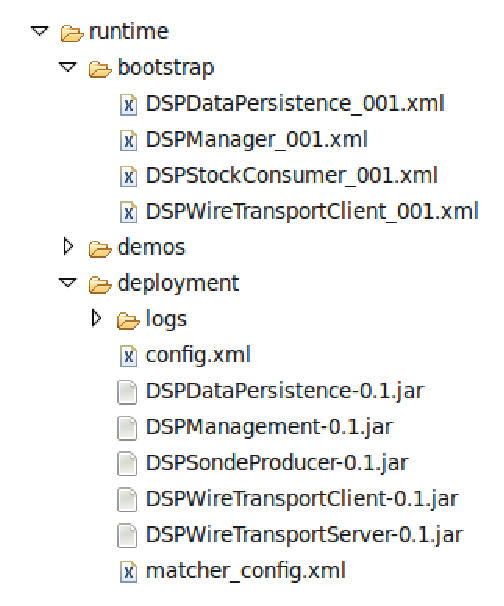
\includegraphics[scale=0.5]{../diagrams/dsp-runtime-dir}
  \caption{The DSP Data Persistence Directory Structure}
  \label{fig:dsp-runtime-dir}
\end{figure}

\section{DSP Platform Deployment}

As described in the previous chapter, the DSP Data Persistence Component was
implemented using the Java Programming language, on top of the osgi-intro Framework
API. This section describes the setup process of the implementation, as well as
the artifacts use during the implementation, which will be listed in the
appendix section.

The structure of the artifacts implemented for the DSP Data Persistence
Component follow the conventions of the NetBEAMS implementation, where the main
directory \textbf{PERSISTENCE-DIR}, depicted by Figure
\ref{fig:dsp-data-persistence-dir-checkedout}, holds each of the development
artifacts.

\begin{itemize}
  \item \textbf{DSPDataPersistence}: Main directory with the build.xml (Listing
  \ref{file:dsp-build.xml}) and other Eclipse-related artifacts. The other
  major directories are also listed:
  \item \textbf{META-INF}: this directory contains the descriptor file for
  the osgi-intro Framework, this this case the MANIFEST.MF;
  \item \textbf{src}: the main directory structure for the source-code
  implemented. Note that it follows the Java specification for packaging, and
  therefore, lists the package org.netbeams.dsp.persistence as the main
  package, including the layers controller, model and osgi-intro.
\end{itemize}

\begin{figure}[!h]
  \centering
  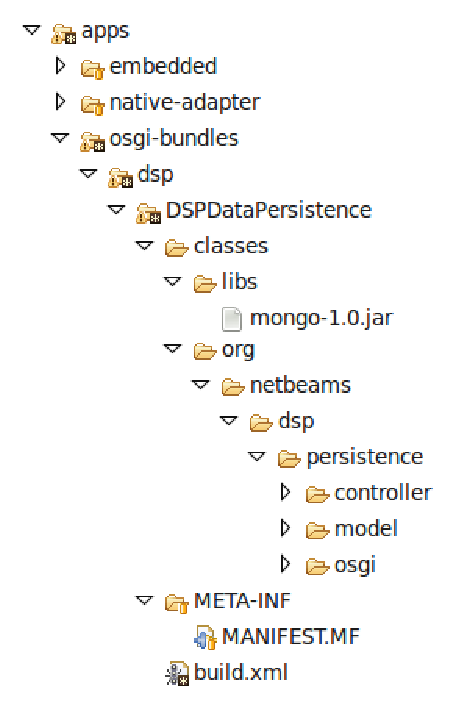
\includegraphics[scale=0.5]{../diagrams/dsp-data-persistence-dir-checkedout}
  \caption{The DSP Data Persistence Directory Structure}
  \label{fig:dsp-data-persistence-dir-checkedout}
\end{figure}

\subsection{osgi-intro Deployment Process}

Since each NetBEAMS component is managed by an osgi-intro component and its
infrastructure, this section describes the basic functionality of the osgi-intro
platform \cite{osgi-intro}, a framework was conceived to support modularity in
terms resources-limited environments such mobile devices and vehicles, but it
was first widely deployed on Eclipe IDE\footnote{Integrated Development
Environment}, because it promotes the use of reusable loosely-coupled modules
using the Java Programming Language \cite{java}. The most basic layer of the
osgi-intro Framework depicted in Figure \ref{fig:layering-osgi-intro} are as follows:

\begin{itemize}
  \item \textbf{Module Layer}: manages the osgi-intro bundles deployed on the osgi-intro
  Platform, providing the necessary "wiring" of the components. In other words,
  the modules, called osgi-intro Bundles, can export and/or import packages in the
  level of a Java Class managed by the osgi-intro Framework;
  \item \textbf{Service Layer}: resposible for the interoperability between 2
  or more bundles, enabling the bundles to register services offered by
  the its specification;
  \item \textbf{Execution Layer}: executes the bundles, managing and changing
  their life-cycle through the bundle execution.
\end{itemize}

\begin{figure}[!h]
  \centering
  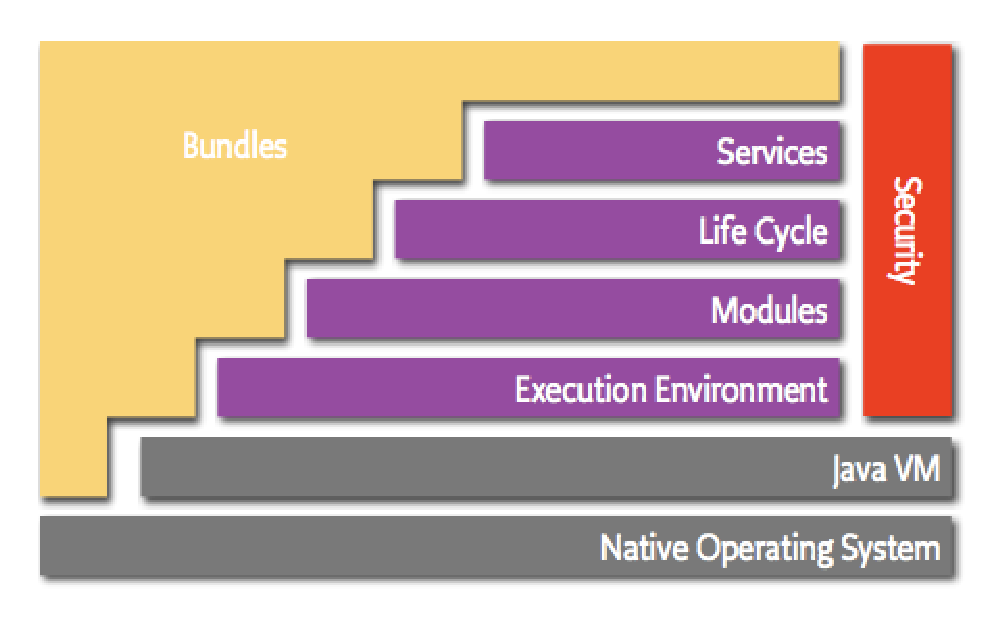
\includegraphics[scale=0.5]{../diagrams/layering-osgi}
  \caption{The osgi-intro Framework Layers}
  \label{fig:layering-osgi-intro}
\end{figure}

NetBEAMS uses the concept of the modularization through the use of the the
Producer-Consumer paradigm described in the previous section. Since the DSP
Components are essentially osgi-intro bundles, the interoperability between them are
given in the implementation and reuse existing bundles in the osgi-intro Framework
and the DSP Platform, described by an artifact called MANIFEST.MF as seen in
listing \cite{file:osgi-intro-manifest}. In general, an osgi-intro bundle must
provide specifications that describes the module to be published into the osgi-intro
Framework. In this way, the main properties of the osgi-intro MANIFEST.MF artifact can
used by the DSP Data Persistence can be summarized as follows:

\begin{itemize}
  \item \textbf{Bundle-Activator}: The name of the instance of an osgi-intro Activator
  class, responsible to manage the bundle. The implemented class
  ``DataPersistenceActivator'' provides the activation mechanisms for the
  services provided by the DSP Data Persistence Component;
  \item \textbf{Bundle-ClassPath}: the necessary Java Jars list needed to run
  the bundle. It lists the mongoDB Java driver as one of the required
  dependencies deployed in the same package;
  \item \textbf{Import-Package}: the Java Packages needed by the DSP Data
  Persistence Component Bundle. These Java Packages must be provided by other
  DSP components, forcing the execution to be dependent on those package.
  They are provided through a ``Export-Package'' section in other osgi-intro
  bundles and, as it is shown in listing \cite{file:osgi-intro-manifest}, they
  are from different packages.
\end{itemize}

Once the osgi-intro bundle is installed into the osgi-intro Platform, it will be managed by
the osgi-intro Execution layer and change the bundle state according to its
lify-cycle, as described in the previous chapter. Therefore, the packaging of
the osgi-intro source-code is done using a JAR\footnote{Java Archival Repository}
artifact specification \cite{java-tutorial}. In this way, the DSP Data
Platform osgi-intro bundle JAR is created by the Apache ANT build script
\cite{apache-ant} in Listing \ref{file:dsp-build.xml}. The task
``dsp-data-persistence.all'' compiles all the source-code created from the
design of the previous chapter and packages everything into the artifact
``DSPDataPersistence-x.x.jar'', where x.x is the version of the bundle. Figure
\ref{fig:dsp-runtime-dir} shows the DSP Data Persistence file under the
dirctory ``\textbf{RUNTIME-DIR}/deployment/''.

\subsection{Adding DSP Data Persistence into DSP Platform }

Once the new component was developed, the DSP Data Persistence component was
deployed by editing two main descriptors, as well as the optional bootstrap
message, as described in chapter 5:

\begin{itemize}
  \item \textbf{config.xml}: the DSP Data Persistence is added to the DSP
  Platform adding an entry for the component;
  \item \textbf{matcher\underline{ }config.xml}: the addition of the rules that
  filters the messages to the DSP Data Persistence;
  \item \textbf{DSPDataPersistence\underline{ }001.xml}: depicts the bootstrap
  message for the DSP Data Persistence Component, as shown in Listing 
  \ref{file:dsp-data-pers-bootstrap.xml}.
\end{itemize}

The first configuration artifact enables NetBEAMS to initialize contain the
descriptor of the component, as shown in Listing \ref{file:dsp-config.xml}.
The component is added with the highest priority, since it contains
dependencies to other DSP Components. 
\subsection{Starting the DSP Platform}

Once the DSP Platform automatically installs all the components described by
the configuration descriptor, the container verifies the dependencies and
starts each of the DSP components of Figure \ref{fig:knopflerfish-execution},
the osgi-intro Framework container Knopflerfish \cite{knopflerfish}.

\begin{figure}[!t]
  \centering
  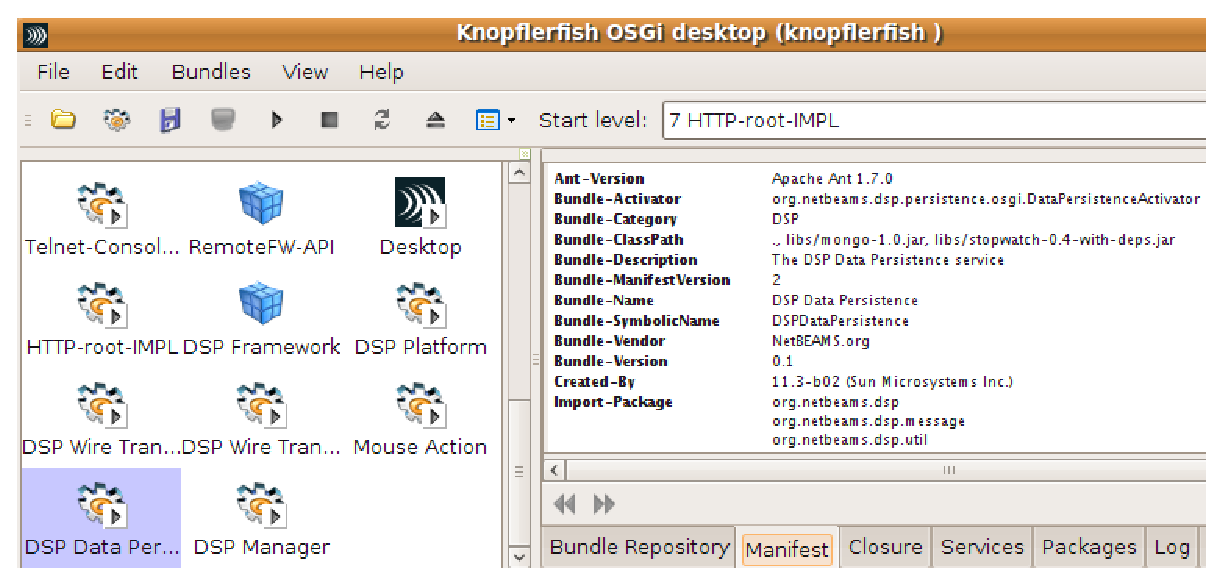
\includegraphics[scale=0.65]{../diagrams/knopflerfish-execution}
  \caption{The execution of the Knopflerfish Container}
  \label{fig:knopflerfish-execution}
\end{figure}

\subsection{Execution Logs}

\section{mongoDB Deployment}

Given that Document-Oriented Model makes a good candidate persist sensors'
properties and the recently enumerated list technologies in the previous
article DSPDataPersistence, the open-source project called mongoDB was chosen
for the evaluation on our case study, the netBEAMS DSP Platform.

mongoDB supports storage based on collections of data, stored using BSON, a
binary representation the JSON data representation format, including dynamic
queries and indexing support. As it's stated in their web site, mongoDB
"bridges the gap between key/value stores (which are fast and highly scalable)
and traditional RDBMS systems (which are deep in functionality)".

\begin{itemize}
  \item mongoDB implements a document-oriented structure, which is similar to
  KVP;
  \item mongoDB is written in C++, and therefore, can is available in any major
  platform, as well as offers a broad range of API drivers written in different
  languages such as Java, Python, Perl and Ruby; 
  \item mongoDB is open-source, with good community support and availability
  through mailing lists, freenode IRC channel, and commercial support through
  10gen company; 
  \item mongoDB has support to distributed systems properties such as
  Master-Slave replication, and features like Database Shards with
  auto-sharding based on shard keys.
\end{itemize}

The artifacts of the mongoDB are located in the thirdparty directory of the
NetBEAMS resources. However, the build script from the DSP Data Persistence
component can be executed to produce the persistence directory
structure for NetBEAMS, as described in figure
\ref{fig:dsp-persistence-system-dir}.

\begin{figure}[!h]
  \centering
  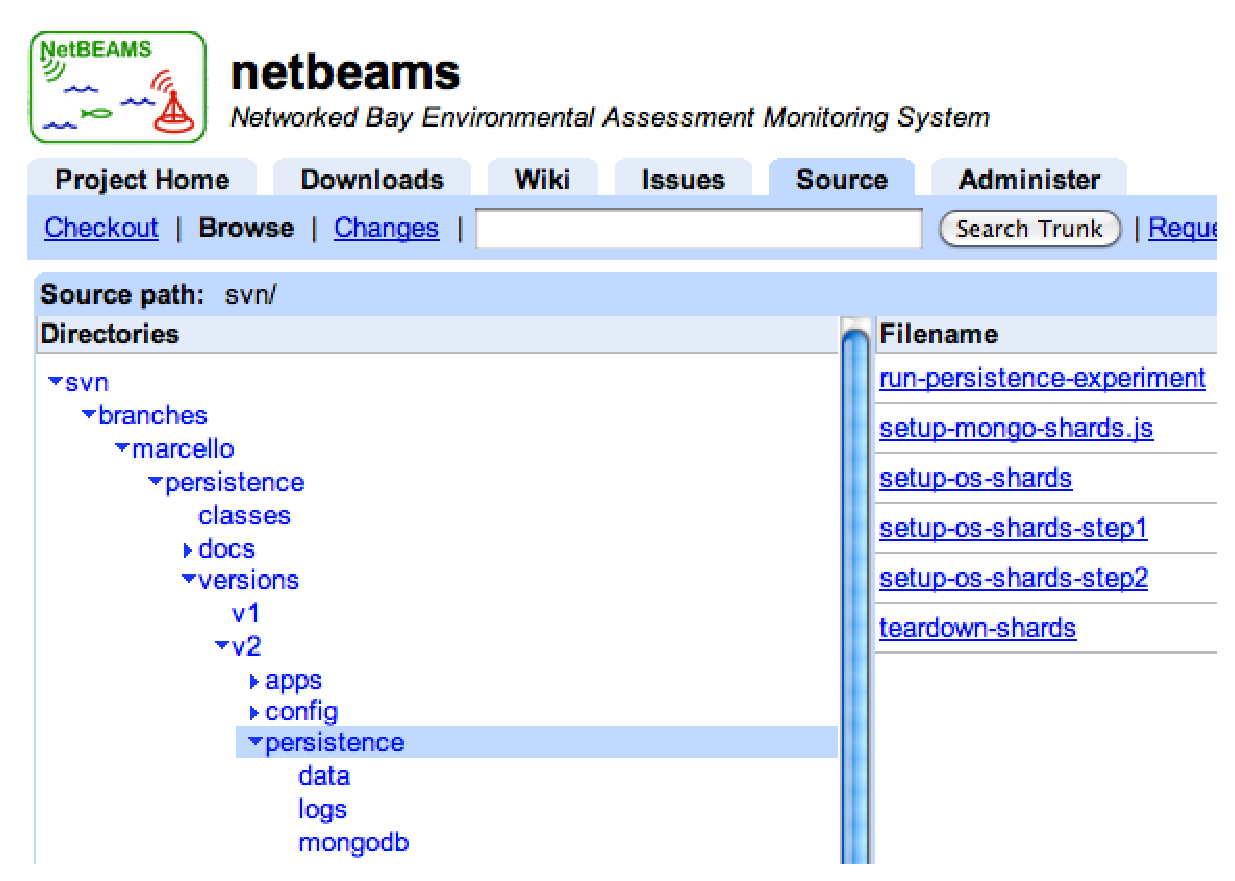
\includegraphics[scale=0.5]{../diagrams/dsp-persistence-system-dir}
  \caption{The osgi-intro Framework Layers}
  \label{fig:dsp-persistence-system-dir}
\end{figure}

Installation of mongoDB
- Explanation about mongoDB processes: mongod, mongos, mongo
- Specification of the shards, shard key, etc

    * The database instance is called "netbeams";
    * The database "netbeams" may contain different collections, categorized by
    the Sensor Content Type, that is, depending on how the DSP Component was
    described;  

\subsection{Document-Oriented Data Model}

An example of the data is as folows (using the JSON syntax). Listing
\ref{file:mongodb-ysi-data-format} follows the strategy described on Section X,
where the entity representation is denormalized, and each of the properties of
the sensor is repeated in each instance of the data. The fact and transaction
times are expressed in milliseconds. The data element contains the complete
structure of the originating sensor such as the IP address. The collection of
instances of this document represents the sensor data type.

\subsection{Starting the Database}

\subsection{Stopping the Database}

\subsection{Execution Logs}

- Java API implementation
- Python API implementation

\section{Data Access Using Database Shell}

The mongoDB client can be started by using the following command. Make sure you
have started the mongoDB server before executing the mongoDB client.

mongo netbeams | tee output\underline{ }number\underline{ }date.log

Here, the iterative mongo client shell offers users to verify and navigate on a
given database and its collections. This first section shows the connection of
the mongo client to the database netbeams. It also highlights the query for the
collections available. During the experiment, the SondeDataContainer?
collection was created as related to the type from the DSP Messages for the YSI
Sonde.

The shell references to the mongoDB system can be found at
http://www.mongodb.org/display/DOCS/dbshell+Reference 

\lstset{label=cmd:mongo,caption=Execution of mongo client}
\begin{lstlisting}
MongoDB shell version: 1.1.0-
url: netbeams
connecting to: netbeams
type "help" for help
> show collections
SondeDataContainer
system.indexes
>
> db.SondeDataContainer.count()
1000000
\end{lstlisting}

Then, the first verification of the data integrity is regarding the number of
elements created. Here, the first count() function on the collection returned
1000000.

An example about retrieving the first element of the collection can be done
using the findOne() function. It will return an element instance on the
JSONnotation.

\lstset{label=cmd:mongo-findone,caption=Querying the database: one item}
\begin{lstlisting}
> db.SondeDataContainer.findOne()
{
    "_id" : ObjectId("5d6f40078ec8074bba980900"),
    "message_id" : "020d82e1-18b2-4fe2-800c-a0f68e22ea86",
    "sensor" : {
        "ip_address" : "192.168.0.91",
        "location" : {
            "latitude" : 37.89155,
            "longitude" : -122.4464
        }
    },
    "time" : {
        "valid" : "Wed Nov 04 2009 02:30:12 GMT-0800 (PST)",
        "transaction" : "Sat Nov 21 2009 03:01:33 GMT-0800 (PST)"
    },
    "observation" : {
        "WaterTemperature" : 88.58,
        "SpecificConductivity" : 180.5,
        "Conductivity" : 167.3,
        "Resistivity" : 491.89,
        "Salinity" : 0.06,
        "Pressure" : 1.109,
        "Depth" : 2.642,
        "pH" : 7.11,
        "pHmV" : -42.9,
        "Turbidity" : 0.2,
        "ODOSaturation" : 72.4,
        "ODO" : 10.85,
        "Battery" : 2.7
    }
}
\end{lstlisting}

The query based on attributes can be done using the "dot" notation, as you
navigate through the JSON documents. Additionally, you can use the functions as
aggregated on the result of others. The example in listing
\ref{cmd:mongo-find-list} counts the number of documents with the key
"data.ph" equals to "5.64".

\lstset{label=cmd:mongo-find-list,caption=Execution of mongo client}
\begin{lstlisting}
> db.SondeDataContainer.find({"data.ph":5.64)}).count()
1226
\end{lstlisting}

The following example is the output of the first 2 documents from the same
previous query using the limit() function, as shown in figure
\ref{cmd:mongo-find-limit}.

\lstset{label=cmd:mongo-find-limit,caption=Query Element with specific
projection limiting the result set size}
\begin{lstlisting}
> db.SondeDataContainer.find({"data.ph":5.64}).limit(2)
{"_id" :  ObjectId( "d36f4007b7e7ac4a03c60000")  , "sensor_ip_address" : "192.168.0.136" , "message_id" : "7b6624d6-0ca1-4cba-a343-f166e88da73b"
, "transaction_time" : 1252845473412 , "fact_time" : 1252845346000 , "data" : {"temperature" : "45.01" , "sp_condition" : "37.6" ,
"condition" : "145.8" , "resistence" : "159.77" , "salinitude" : "0.0" , "pressure" : "0.391" , "depth" : "0.46" , "ph" : "5.64" ,
"pH_mv" : "-62.1" , "odo_sat" : "89.7" , "odo_condition" : "59.34" , "turbidity" : "0.0" , "battery" : "9.4"}}
{"_id" :  ObjectId( "d36f4007b7e7ac4a1fc80000")  , "sensor_ip_address" : "192.168.0.136" , "message_id" : "7b6624d6-0ca1-4cba-a343-f166e88da73b" ,
"transaction_time" : 1252845473412 , "fact_time" : 1252845346000 , "data" : {"temperature" : "46.71" , "sp_condition" : "60.8" ,
"condition" : "160.6" , "resistence" : "1399.4" , "salinitude" : "0.01" , "pressure" : "1.057" , "depth" : "2.485" , "ph" : "5.64" ,
"pH_mv" : "-16.3" , "odo_sat" : "58.8" , "odo_condition" : "19.29" , "turbidity" : "0.2" , "battery" : "9.2"}}
>
\end{lstlisting}

Other logs are located at
http://code.google.com/p/netbeams/downloads/list

\section{Data Access Using APIs}

The mongoDB server offers different drivers to access the data, as well as the
Web Services.

\begin{itemize}
  \item The Java tutorial on the drivers is located at
    http://www.mongodb.org/display/DOCS/Java+Tutorial. The driver is located on
    the NETBEAMS/versions/v2/thirdparty/mongodb directory;  
  \item The REST API can be called from any HTTP client. At the time of the
  editing, this feature is still under alpha version. Check the documentation
  athttp://www.mongodb.org/display/DOCS/Http+Interface for details 
\end{itemize}

The following HTTP GET Request method returns the first 5 documents in the collection:
http://127.0.0.1:28017/netbeams/SondeDataContainer/?limit=-5, as shown in
listing \ref{cmd:mongo-rest-request}.

\lstset{label=cmd:mongo-rest-request,caption=REST HTTP GET Request Example}
\begin{lstlisting}
HTTP/1.0 200 OK
x-action:
x-ns: netbeams.SondeDataContainer
Content-Type: text/plain;charset=utf-8

{
  "offset" : 0,
  "rows": [
    { "_id" : "156f4007e4c3b74a36ed3100", "sensor_ip_address" : "192.168.0.117", "message_id" : "08b02c08-9290-4517-9a28-c6ee7e16509a",
"transaction_time" : 1253557219486, "fact_time" : 1253557217000, "data" : { "temperature" : "31.44", "sp_condition" : "99.8", "condition" : "53.5",
"resistence" : "1157.08", "salinity" : "0.0", "pressure" : "1.066", "depth" : "0.161", "ph" : "1.08", "pH_mv" : "-82.0", "odo_sat" : "40.3",
"odo_condition" : "56.85", "turbidity" : "0.2", "battery" : "8.2" } } ,
    { "_id" : "156f4007e5c3b74a37ed3100", "sensor_ip_address" : "192.168.0.117", "message_id" : "08b02c08-9290-4517-9a28-c6ee7e16509a",
"transaction_time" : 1253557219486, "fact_time" : 1253557217000, "data" : { "temperature" : "37.83", "sp_condition" : "176.3", "condition" : "2.6",
"resistence" : "1324.97", "salinity" : "0.01", "pressure" : "1.36", "depth" : "1.564", "ph" : "0.12", "pH_mv" : "-23.5", "odo_sat" : "104.5",
"odo_condition" : "19.44", "turbidity" : "0.1", "battery" : "5.0" } } ,
    { "_id" : "156f4007e5c3b74a38ed3100", "sensor_ip_address" : "192.168.0.117", "message_id" : "08b02c08-9290-4517-9a28-c6ee7e16509a",
"transaction_time" : 1253557219486, "fact_time" : 1253557217000, "data" : { "temperature" : "74.3", "sp_condition" : "84.0", "condition" : "104.7",
"resistence" : "4089.13", "salinity" : "0.01", "pressure" : "1.222", "depth" : "2.788", "ph" : "6.56", "pH_mv" : "-78.1", "odo_sat" : "40.0",
"odo_condition" : "6.02", "turbidity" : "0.3", "battery" : "3.2" } },
  "total_rows" : 3 ,
  "query" : {} ,
  "millis" : 0
}
\end{lstlisting}

Data visualisation tools for mongoDB is slowly being developed by open-source
developers. The next picture shows the database "netbeams" and the collection
"SondeDataContainer  ?" being rendered by futon4mongodb, one of the
open-source tools developed to visualise mongoDB data.

\section{Visualizing Data on The Browser}

Futon4Mongo is an open-source software adapted from CouchDB \ref{couchdb}.
First, the collections list is shown. Figure
\ref{fig:view-collections-instance-browser-futondb} shows one single collection
for the YSI data containing 1 million objects.

\begin{figure}[h]
  \centering
  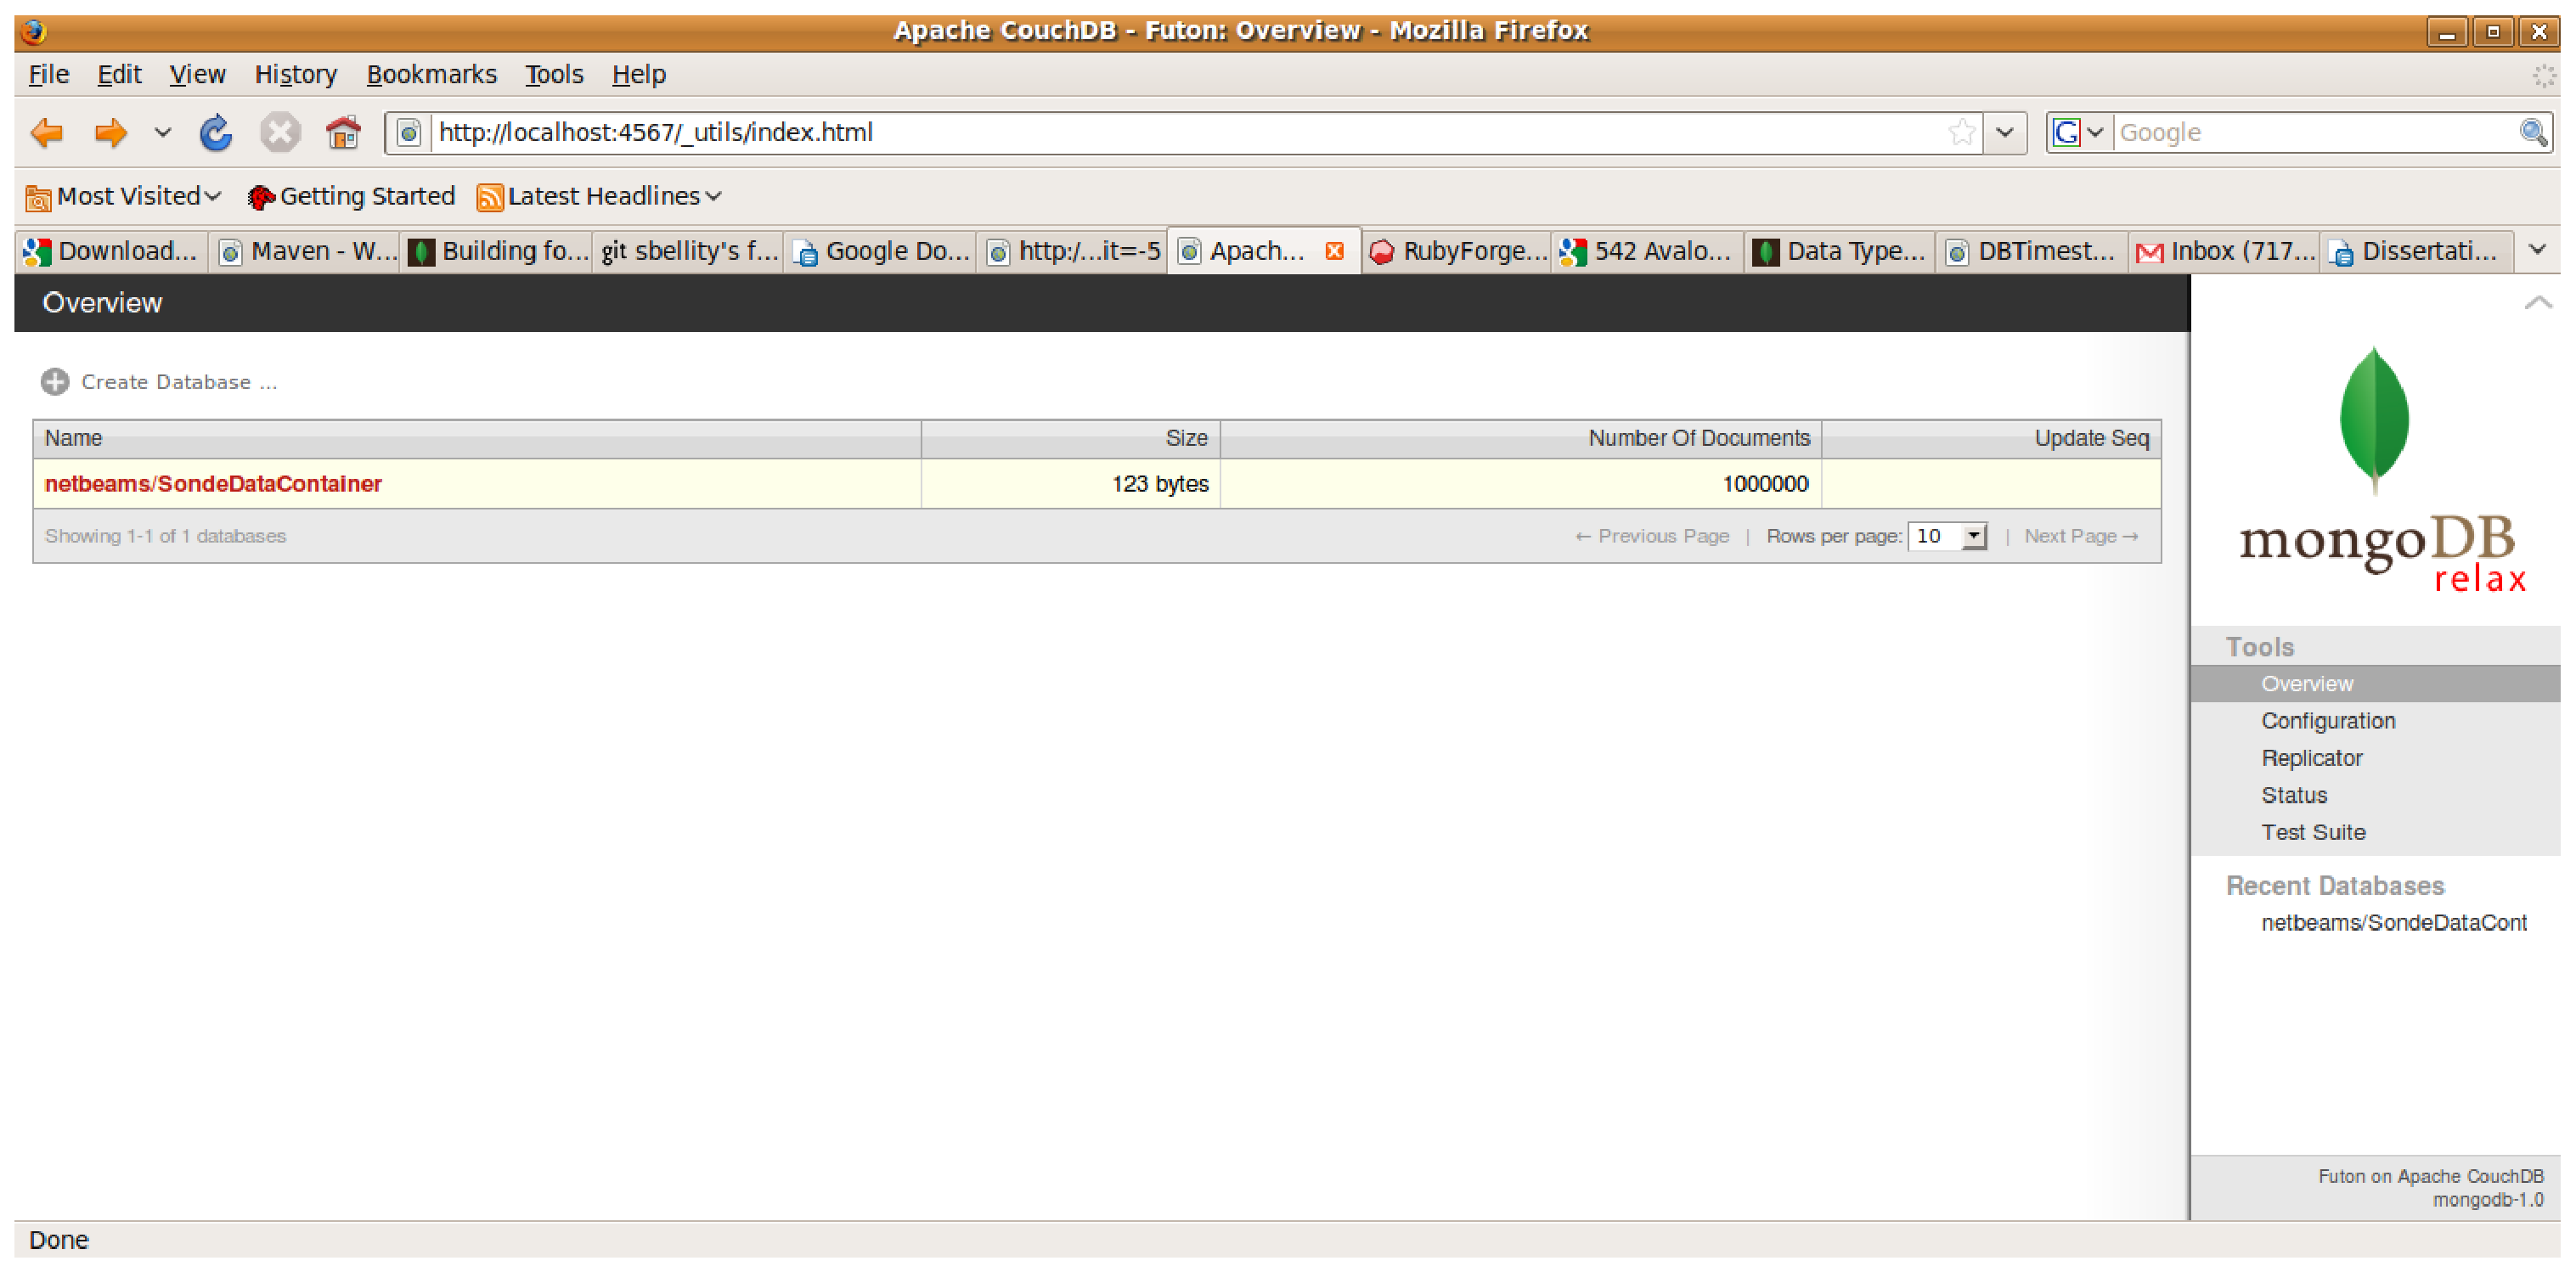
\includegraphics[scale=0.3]{../diagrams/view-collections-instance-browser-futondb}
  \caption{Viewing a partial list of data using the Futon for CouchDB/MongoDB}
  \label{fig:view-collections-instance-browser-futondb}
\end{figure}

The collection is composed by instances of documents of representing the YSI
Sonde type, being indexed by a document ID and the values being the keys
defined in the previous chapter, as shown in figure
\ref{fig:view-collected-data-list-browser-futondb}.

\begin{figure}[h]
  \centering
  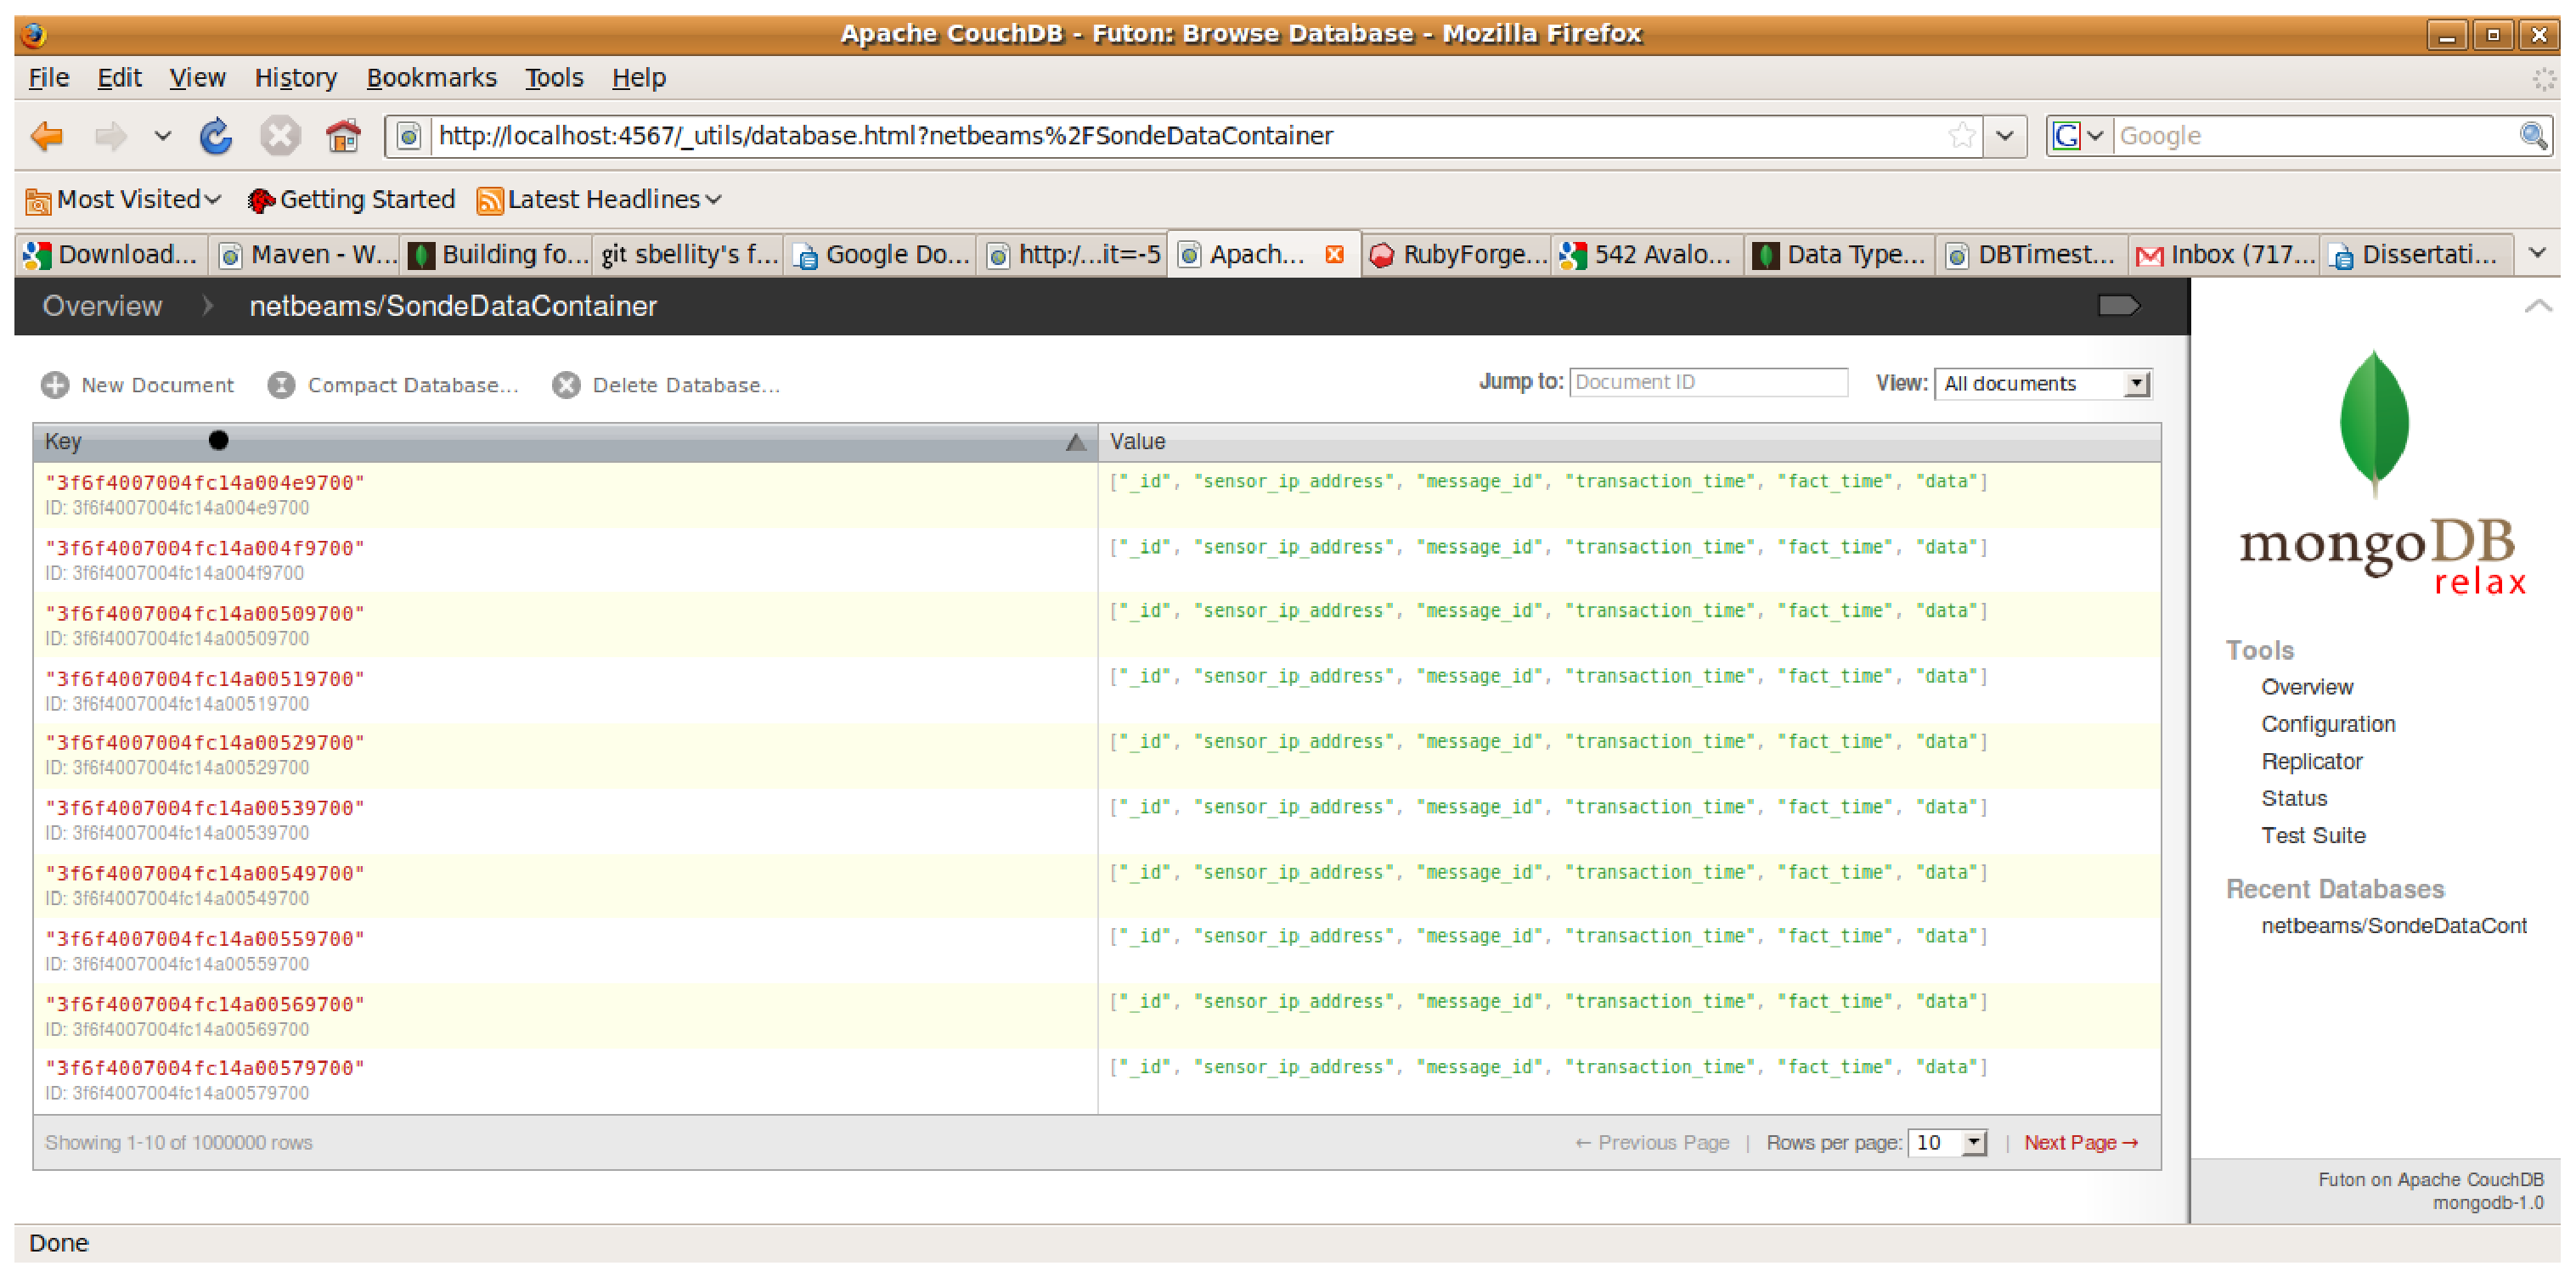
\includegraphics[scale=0.3]{../diagrams/view-collected-data-list-browser-futondb}
  \caption{Viewing a partial list of data using the Futon for CouchDB/MongoDB}
  \label{fig:view-collected-data-list-browser-futondb}
\end{figure}

By clicking in one of the items, one can view the instance of the document, as
it is shown in figure \ref{fig:view-collections-instance-browser-futondb}.

\begin{figure}[h]
  \centering
  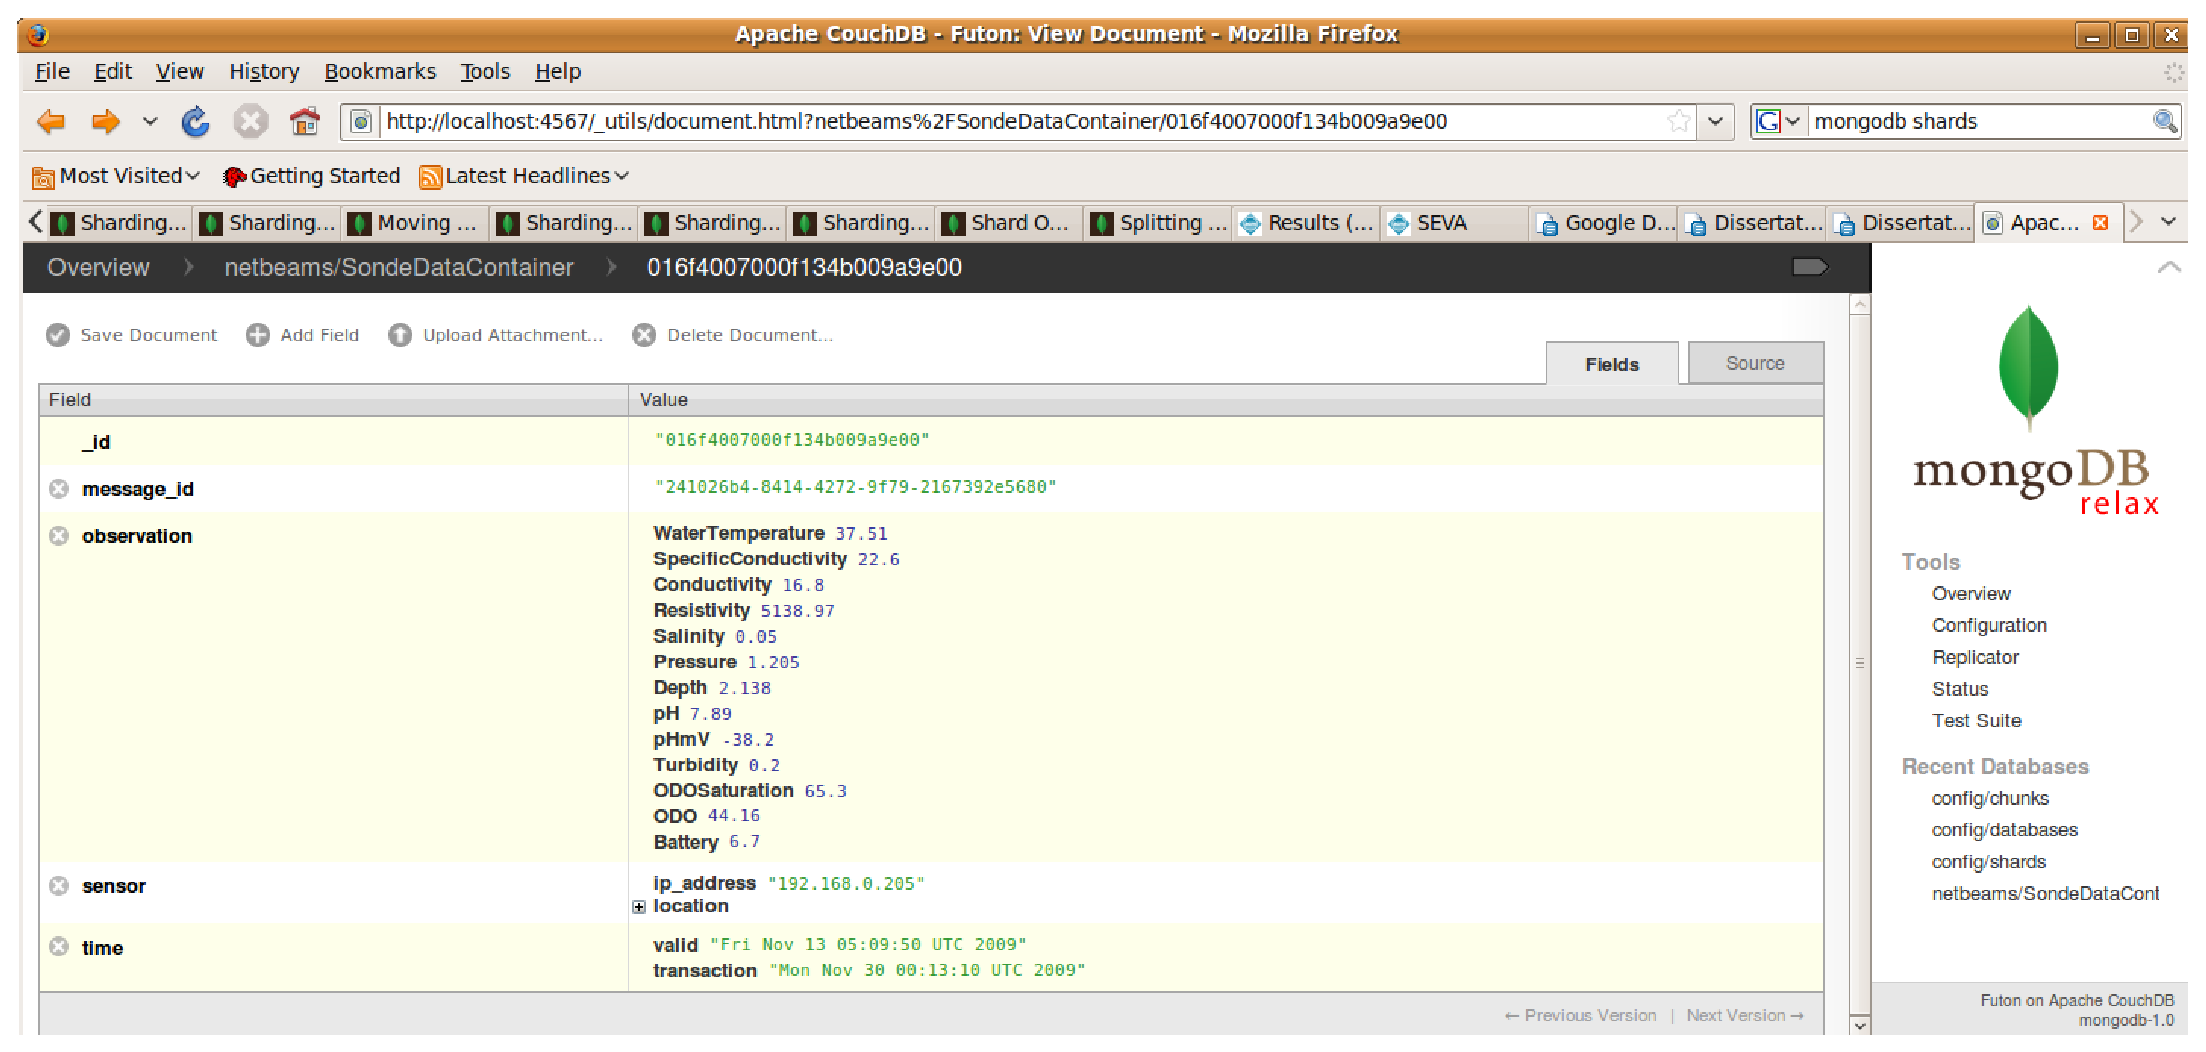
\includegraphics[scale=0.3]{../diagrams/view-collected-data-instance-browser-futondb}
  \caption{Viewing an instance of collected data using the Futon for
  CouchDB/MongoDB}
  \label{fig:view-collected-data-instance-browser-futondb}
\end{figure}

\section{Exporting Data to Spreadsheets}

mongoDB has an export facility shell called mongoexport. It can export the data
in JSON format or CSV. One may also write its own export tool in any of the
languages such as Java, PHP, Python, Perl, Ruby, among others. A list of the
existing drivers in different languages is provided
athttp://www.mongodb.org/display/DOCS/Drivers. The following command can be
executed to have the exported version of the data in CSV (read the help output
of the command for details).

An example to export the data in CSV format can be seen in listing
\ref{cmd:mongoexport}, and an example containing 1 million objects can be
downloaded at
http://netbeams.googlecode.com/files/experiment-1000000-data-exported-20090913-053538.csv.tar.gz.

\lstset{label=cmd:mongoexport,caption=Command to export data in CSV format}
\begin{lstlisting}
mongoexport -d netbeams -c SondeDataContainer --dbpath ./data/ --csv -f "_id,sensor_ip_address,transaction_time,fact_time,
data.temperature,data.sp_condition,data.condition,data.resistence,data.salinitude,data.pressure,data.depth,data.ph,data.pH_mv,data.odo_sat,
data.odo_condition,data.turbidity,data.battery" -o sonde-data-exported.csv
\end{lstlisting}

\section{Exporting Data to OPeNDAP Format}

By using any programming language driver, one can export data in the OPeNDAP
format.